\documentclass[conference]{IEEEtran}
\IEEEoverridecommandlockouts
% The preceding line is only needed to identify funding in the first footnote. If that is unneeded, please comment it out.
\usepackage{cite}
\usepackage{amsmath,amssymb,amsfonts}
\usepackage{algorithmic}
\usepackage{graphicx}
\usepackage{textcomp}
\usepackage{xcolor}
\usepackage{tikz}
\usetikzlibrary{positioning}
\def\BibTeX{{\rm B\kern-.05em{\sc i\kern-.025em b}\kern-.08em
    T\kern-.1667em\lower.7ex\hbox{E}\kern-.125emX}}
\begin{document}

\title{Guitar Percussive Classification for Effect Control\\

}

\author{\IEEEauthorblockN{Oliver Whorwood}
\IEEEauthorblockA{\textit{School of Electronic Engineering and Computer Science} \\
\textit{Queen Mary University of London}\\
London, UK \\
ec21904@qmul.ac.uk}
}

\maketitle

\begin{abstract}

\end{abstract}
 
 



\section{Introduction}
This paper outlines the design and development of a guitar percussive classification system for parameter control of effects. This need for such a system stems from a proposed
requirement from HyVibe who manufacture a guitar amplification system which uses actuators placed onto a guitar body.

The system is based around a deep learning algorithm that is trained on a large dataset of guitar percussive signals. 

A piezoelectric pickup underneath the saddle of a guitar produces a small electrical signal which is amplified to line level for use by the classification system.

This real-time classification system is built on Python and is used to recognize control taps and send a MIDI message to the controller to change certain parameters.

The system is evaluated using subjective measures such as F-measure for the offline system, and recall accuracy when using the system as intended.

The aim is to have a system that can detect 2 different types of control taps to send out 2 different control messages when the user is playing normal plucked or strummed guitar simultaneously.


\section{Literature review}

\subsection{Percussive classification}

In a review of current onset detection techniques, modern approaches of using a Convolutional Neural Network (CNN) such as with image classification are shown to be more efficient than 
more traditional methods such as High Frequency Content or Recurrent Neural Networks (RNNs) \cite{b2}.

An efficient CNN based approach for onset detection has been proposed \cite{b1} which uses two convolutional filters followed by a fully connected layer. This method is used to detect
downbeat positions in a range of genres of music and outperforms other competing methods such as RNN and SuperFlux. The F-measure of the CNN system is 0.885 compared to 0.873 for RNN. This
is shown to be improved upon further by adding dropout, something which needs to be considered here, especially with a small dataset which can suffer from overfitting \cite{b8}.

For detecting specific patterns of onsets, the system will require an internal 'memory' to create a causal system. This is commonly achieved using an LSTM layer combined with CNN \cite{b6}, with this paper in
particular focussing on its use for music emotion recognition. Another pattern recognition option is the use of CRNNs as described in \cite{b7}, which combines the local features of CNNs with temporal features of RNNs.

The latency of the system needs to be low enough to not have a detrimental effect on playability. For musicians even a delay of 10ms between musical beats \cite{b4} is noticeable. This paper however
focusses on musical latency whereas the system proposed will be used for control of effects, so the tolerance may well be higher. 

The parts of the guitar that are focussed on are the front body, divided into the lower and upper bout, the saddle, and the side \cite{b3}. The positions of these can be seen in ``Fig.~\ref{guitar}'.

\begin{figure}[htbp]
    \centerline{\includegraphics[scale=0.4]{guitar.png}}
    \caption{Labelled parts of an acoustic guitar. \cite{b3}}
    \label{guitar}
    \end{figure}


\section{Methodology}
There are many sections of a guitar which can be struck to produce a sound. These can be split into harmonic and inharmonic components, the strings produce harmonic content when
struck whereas the body of the guitar produces inharmonic content. The harmonicity refers to the relationship of frequencies where there are integer multiples of the fundamental frequency.
Many guitar players also use the inharmonic components to act as percussion. 

To test the feasibility of such a classification system, a prototype was developed to recognize the onsets of three positions of tapping in real time and send one MIDI message to the HyVibe system.
The three tapping locations are: the saddle board, the lower bout and the underside of the guitar.
The initial system is trained using three audio files, each of the three tapping locations. There are 100 taps per audio file spaced at 1 second intervals. As the intervals are not
exact, the location of the taps are manually annotated, producing a text file with a list of the tap locations in seconds.

The signal is first converted to the frequency domain via a Short-Time Fourier Transform (STFT) with a window size of 2048 samples and a hop size of 512 samples using the 'librosa' Python library. The output is split
into sections of 15 windows wide creating input data with 15375 values each with a corresponding ground truth of an integer 0-2. The training set is a random selection of 80\% of this dataset with a remaining 20\% reserved for offline testing. 
The output of the neural network is a multi-class softmax function. If a threshold of 0.5 is reached for class 1 (a control tap), then a MIDI message of type 'note-off' is sent to the HyVibe system over 
Bluetooth Low Energy (BLE).

The full neural network is: convolution (3x7) with 10 features, maxpool (3x1), convolution (3x3) with 20 features, maxpool (3x1), flatten, Dense (256), Dense (3).

The real time detection system is written in Python and subsequently sends serial messages to an ESP32 development board which is programmed in C++ to send a MIDI BLE message when a serial
message of `1' is received.

\begin{figure}[htbp]
    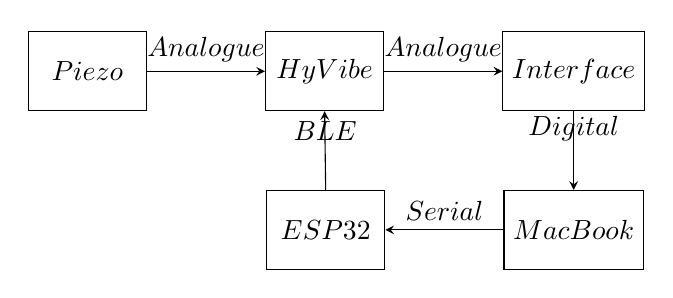
\begin{tikzpicture}
     
    \node[draw,
        minimum height=1cm,
        minimum width=1.5cm,
        fill=white]
        (piezo) at (0,0){$Piezo$};
    
    \node[draw,
        minimum height=1cm,
        minimum width=1.5cm,
        right=1.5cm of piezo,
        fill=white]
        (hyvibe) {$HyVibe$};
    
    \node[draw,
        minimum height=1cm,
        minimum width=1.5cm,
        right=1.5cm of hyvibe,
        fill=white]
        (interface) {$Interface$};
    
    \node[draw,
        minimum height=1cm,
        minimum width=1.5cm,
        below=1cm of interface,
        fill=white]
        (macbook) {$MacBook$};
    
    \node[draw,
        minimum height=1cm,
        minimum width=1.5cm,
        left=1.5cm of macbook,
        fill=white]
        (esp) {$ESP32$};
    
    \draw[-stealth] (piezo.east) -- (hyvibe.west)
        node[midway,above]{$Analogue$};
    
    \draw[-stealth] (hyvibe.east) -- (interface.west)
        node[midway,above]{$Analogue$};
    
    \draw[-stealth] (interface.south) -- (macbook.north)
        node[midway,above]{$Digital$};
    
    \draw[-stealth] (macbook.west) -- (esp.east)
        node[midway,above]{$Serial$};
    
    \draw[-stealth] (esp.north) -- (hyvibe.south)
        node[midway,above]{$BLE$};
     
    \end{tikzpicture}
    \caption{An overview of the system architecture.}
    \label{system}
    \end{figure}

\section{Results \& Discussion}

The results of the initial prototype are promising, although this represents an ideal scenario with no other noise and only three tap locations. For the offline system, this has an
average F-measure of 0.99.

The online system is also tested for latency in three scenarios, first triggered by an onset tap, then from a keyboard press from Python, and finally a button press directly from the
ESP32 board. The latency for the fist scenario is measured by recording the audio output and measuring the time difference between the first audio peak in the onset and the first audio peak in the metronome. The second 
scenario is measured by sending a MIDI message on the keyboard press which is recorded alongside the audio output. For the third scenario the button is pressed at the same time as a note on a MIDI keyboard. 
Each scenario is tested 5 times and the average latency is calculated. For the onset trigger, the total latency is a fairly substantial 1167.4ms. Comparing this with sending
the serial message directly from the Python script via a keyboard press, the latency is 1037.4ms. Finally, when the button is used, the latency is less than 1ms.
There is a serious bottleneck in the system at the serial communication layer. The onset detection itself only accounts for an average of 130ms of latency. Other methods to relay the signal
from Python may have to be considered.


\begin{thebibliography}{00}
\bibitem{b1} J. Schlüter and S. Böck, ``Improved musical onset detection with Convolutional Neural Networks,'' 2014 IEEE International Conference on Acoustics, Speech and Signal Processing (ICASSP), 2014, pp. 6979-6983, doi: 10.1109/ICASSP.2014.6854953.
\bibitem{b2} C. -W. Wu et al., ``A Review of Automatic Drum Transcription,'' in IEEE/ACM Transactions on Audio, Speech, and Language Processing, vol. 26, no. 9, pp. 1457-1483, Sept. 2018, doi: 10.1109/TASLP.2018.2830113.
\bibitem{b3} C. Bay, ``Glossary of Guitar Terms,'' Mel Bay Publications, 2013.
\bibitem{b4} R.H. Jack, A. Mehrabi, T. Stockman and A. McPherson, ``Action-sound latency and the perceived quality of digital musical instruments: Comparing professional percussionists and amateur musicians.'' Music Perception: An Interdisciplinary Journal, 36(1), pp.109-128, 2018.
\bibitem{b5} M. A. Rohit, A. Bhattacharjee and P. Rao, ``FOUR-WAY CLASSIFICATION OF TABLA STROKES WITH MODELS ADAPTED FROM AUTOMATIC DRUM TRANSCRIPTION'', 22nd ISMIR Conference, Nov. 2021.
\bibitem{b6} Y. Yu, ``Research on Music Emotion Classification Based on CNN-LSTM Network,'' 2021 5th Asian Conference on Artificial Intelligence Technology (ACAIT), 2021, pp. 473-476, doi: 10.1109/ACAIT53529.2021.9731277.
\bibitem{b7} Z. Wang, S. Muknahallipatna, M. Fan, A. Okray and C. Lan, ``Music Classification using an Improved CRNN with Multi-Directional Spatial Dependencies in Both Time and Frequency Dimensions,'' 2019 International Joint Conference on Neural Networks (IJCNN), 2019, pp. 1-8, doi: 10.1109/IJCNN.2019.8852128.
\bibitem{b8} N. Srivastava, G. Hinton, A. Krizhevsky, I. Sutskever and R. Salakhutdinov. ``Dropout: a simple way to prevent neural networks from overfitting.'' J. Mach. Learn. Res. 15, 1 (January 2014), 1929–1958, 2014.

\end{thebibliography}
\vspace{12pt}

\end{document}
